% llm-prof: Decoupling Continuous Profiling Bandwidth from Sampling Rate
% USENIX ATC-style paper (template: usenix2019_v3.1 / usenix-2020-09.sty)
% Compile: pdflatex paper.tex && pdflatex paper.tex

\documentclass[letterpaper,twocolumn,10pt]{article}
\usepackage{usenix-2020-09}
\usepackage{graphicx}
\usepackage{booktabs}
\usepackage{amsmath}
\usepackage{hyperref}

\begin{document}

%-------------------------------------------------------------------------------
\title{\bf \Large Kernel-Side Streaming Stack Compression for Continuous
Profiling: Decoupling Bandwidth from Sampling Rate}

\author{
{\rm llm-prof Team}\\
{\rm ai-infra}
}

\maketitle

%-------------------------------------------------------------------------------
\begin{abstract}
Continuous profiling of large-scale AI workloads demands high sampling rates
($\geq$1\,kHz per CPU) to capture short-lived hotspots, GIL contention, and
off-CPU waits. eBPF-based samplers make such rates affordable on the CPU side
($<$3\% overhead at 10\,kHz), but the data path does not scale: every sample
carries its full stack, so ringbuffer bandwidth grows linearly with the
sampling rate. At 10\,kHz a single process already produces 3.95\,MB/s;
aggregating profilers (e.g., Parca) recover bandwidth only by discarding
per-sample temporal information, and the kernel's own stack-dedup helper
(\texttt{bpf\_get\_stackid}) hashes \emph{raw} addresses with a lossy 32-bit
signature.

We present the design, implementation, and evaluation of kernel-side streaming
stack compression for \emph{post-unwind} mixed stacks (Python\,$+$\,native):
an incremental 64-bit fingerprint folded while the stack is unwound, an LRU
stack dictionary in eBPF, and a 40-byte \textsc{StackIDEvent} that replaces the
full trace for already-seen stacks. Because the fingerprint is the key,
kernel LRU eviction is trivially safe---an evicted stack simply reverts to
full samples---and userspace re-expands events from a bounded cache, keeping
the aggregation path identical to the uncompressed mode. The key insight is
that unwind output is \emph{already normalized} (\texttt{fileID, offset}):
ASLR is eliminated at unwind time, so compression needs no symbolization.

On six workloads spanning single-hotspot loops, GIL contention, I/O-bound
loops, LLM-style training loops, and deep high-cardinality stacks, compressed
bandwidth is 53--75\% lower at 1\,kHz and 94.6\% lower at 10\,kHz, while the
bandwidth-vs-rate curve flattens from 56$\times$ (uncompressed) to 6$\times$
(compressed) growth. Sample counts and stack sets match the uncompressed path
($\pm$5\%), and the CPU cost of compression is below measurement noise
($<$0.5\,pp at 10\,kHz). We also characterize the compression boundary: the
gain is governed by the stack distribution shape (distinct/sample ratio),
which we can predict from a data-profile, making the ``useless regime''
(e.g., deep stacks, only 2.5\% reduction) a predictable, documented property
rather than a surprise.
\end{abstract}

%-------------------------------------------------------------------------------
\section{Introduction}

Continuous profiling is becoming standard infrastructure for large-scale
AI training and inference clusters \cite{parca,pyroscope,otelprof}: operators
need to attribute latency and utilization to code paths across Python, C++,
and CUDA. LLM workloads make this especially demanding. Training loops
alternate between I/O waits, compute, and synchronization on sub-millisecond
time scales; inference has distinct prefill/decode phases; and both exhibit
GIL contention that classic ptrace-based profilers not only measure poorly
but actively perturb---py-spy at 1\,kHz inflates GIL waits by up to 16$\times$
on our workloads (Section~\ref{sec:motive}).

eBPF-based samplers remove the CPU-side barrier: llm-prof (our system)
profiles Python\,$+$\,native\,$+$\,kernel mixed stacks at 10\,kHz with
$<$3\% CPU overhead, versus 18--81\% for ptrace-based tools at the same rate.
But the \emph{data path} does not scale. Every sample carries its full
unwound stack (0.5--1\,KB), so ringbuffer bandwidth grows linearly with the
sampling rate: 0.07\,MB/s at 100\,Hz, 0.43\,MB/s at 1\,kHz, 3.95\,MB/s at
10\,kHz for a single process. Multiplied across a cluster, and compounded by
userspace parsing and symbolization, this bandwidth wall is the reason
production profilers either cap sampling rates or aggregate in the kernel.

Existing escapes are unsatisfactory. Aggregating profilers such as Parca
count stacks in the agent and export only aggregates, discarding per-sample
timestamps and event fidelity. The kernel's \texttt{bpf\_get\_stackid}
helper deduplicates \emph{raw address} stacks with a lossy 32-bit hash and no
consistency protocol. pprof-level compression happens too late, after the
data has crossed the kernel-userspace boundary.

\paragraph{Key insight.}
Our unwind output is \emph{already normalized}: native frames are
\texttt{(fileID, offset)} and Python frames are \texttt{(fileID, lineno)}
---ASLR is eliminated at unwind time, so the frame sequence is a stable key
without any symbolization. And real workloads make the key highly repetitive:
on our LLM-style training loop, the top-20 stacks cover 80\% of samples, and
a single-hotspot loop has 155:1 sample-to-distinct-stack redundancy. This
means a kernel-side stack dictionary can replace most full traces with a
40-byte event carrying a fingerprint and a count---bandwidth becomes
proportional to \emph{stack churn}, not sampling rate.

\paragraph{Contributions.}
\begin{itemize}
\item \textbf{C1: A kernel-side streaming compression protocol for post-unwind
mixed stacks.} Incremental 64-bit fingerprints folded during unwinding
(verifier-friendly, $\sim$6 instructions per frame), an LRU stack dictionary
in eBPF, and a 40-byte \textsc{StackIDEvent} that preserves
\texttt{ktime/pid/tid/count}---the per-sample stream is retained, unlike
aggregating profilers.
\item \textbf{C2: Correctness by construction.} The fingerprint \emph{is}
the key, so LRU eviction is safe (an evicted stack reverts to full samples);
userspace re-expands events from a bounded cache whose capacity matches the
kernel dictionary, keeping the aggregation path byte-identical to the
uncompressed mode. C and Go implementations of the fingerprint are locked by
a fixed-vector cross-language test.
\item \textbf{C3: Measured end-to-end.} 53--75\% bandwidth reduction across
six workloads at 1\,kHz, 94.6\% at 10\,kHz; the bandwidth-vs-rate curve
flattens from 56$\times$ to 6$\times$ growth; sample counts and stack sets
match the uncompressed path; compression CPU cost is below measurement noise.
\item \textbf{C4: A predictable compression boundary.} The gain is governed
by the stack distribution shape (distinct/sample ratio), formalized as a
dictionary amortization model; we measure the zero-gain regime (deep stacks:
2.5\%) and show it is predictable from data profiling.
\end{itemize}

%-------------------------------------------------------------------------------
\section{Background and Motivation}
\label{sec:motive}

\subsection{The profiling pipeline and its costs}
A continuous profiler is a pipeline of four stages: \emph{collect}
(sampling timer $\rightarrow$ unwinding), \emph{transfer} (ringbuffer
kernel$\rightarrow$userspace), \emph{process} (decode, symbolize, aggregate),
and \emph{store} (pprof/series storage). Each sample costs
$T_\text{sample} = T_\text{intr} + \sum_\text{frames} c_\text{unwind}$, where
$T_\text{intr}\approx2\,\mu$s is the interrupt entry/exit cost (measured by
rate-scaling experiments) and unwinding is roughly $0.3\,\mu$s per frame.
The transfer cost is $B = \text{rate} \times N_\text{CPU} \times
E[\text{send\_size}]$: ringbuffer bandwidth grows linearly with rate.

\subsection{Why high sampling rates matter for LLM workloads}
Short-lived phenomena dominate LLM performance: GIL contention, data-loader
I/O waits, synchronization points in training loops, and prefill/decode
phase transitions. The sampling theorem analog applies: an event is
observable only if sampled while active, so capturing sub-millisecond waits
requires kHz rates. Empirically, 1\,kHz is the minimum useful rate, and
10\,kHz materially improves capture of short stacks. ptrace-based profilers
make this expensive: py-spy at 1\,kHz adds 18--81\% CPU overhead on our
workloads and distorts GIL measurements (the observer effect). eBPF samplers
run at 10\,kHz with $<$3\% overhead---the CPU side is solved.

\subsection{The bandwidth wall}
The unsolved cost is transfer. \texttt{llm-prof} allocates its ringbuffer
as $\text{rate}\times N_\text{CPU}\times\text{sizeof(Trace)}$ (25.3\,KB,
dominated by the 24\,KB frame array); at 10\,kHz $\times$ 16 CPUs this
exceeds the 2\,GB cap. Actual production rates are lower but still linear:
we measure 0.07 / 0.43 / 3.95\,MB/s at 100 / 1k / 10k\,Hz for a single
process. The data is also highly redundant: identical stacks recur
constantly. Figure~\ref{fig:bandwidth} (top line) shows the linear wall;
the bottom line shows what this paper's compression achieves.

\subsection{Data profile: stacks are Zipf, converged, and stable}
We instrumented our sampler with a raw sample-stream export and measured
address-level stack distributions. Three facts
drive the design. \textbf{(a) Zipf concentration:} the top-20 stacks cover
70--80\% of samples on our workloads; a single-hotspot loop has
155:1 sample-to-distinct redundancy, and even the LLM training loop
(\texttt{train\_torch}) shows 6.3:1 (Figure~\ref{fig:profile}a).
\textbf{(b) Convergence:} distinct
stacks accumulate quickly and then saturate---the dictionary warm-up cost is
paid once. \textbf{(c) Frame stability:} even ``unsigned'' frames (JIT/anonymous
code, 20\% of frames on the torch workload) have highly stable addresses
within a run (1{,}498 frames, only 122 distinct values), so they participate
in the dictionary normally.

\begin{figure}[t]
\centering
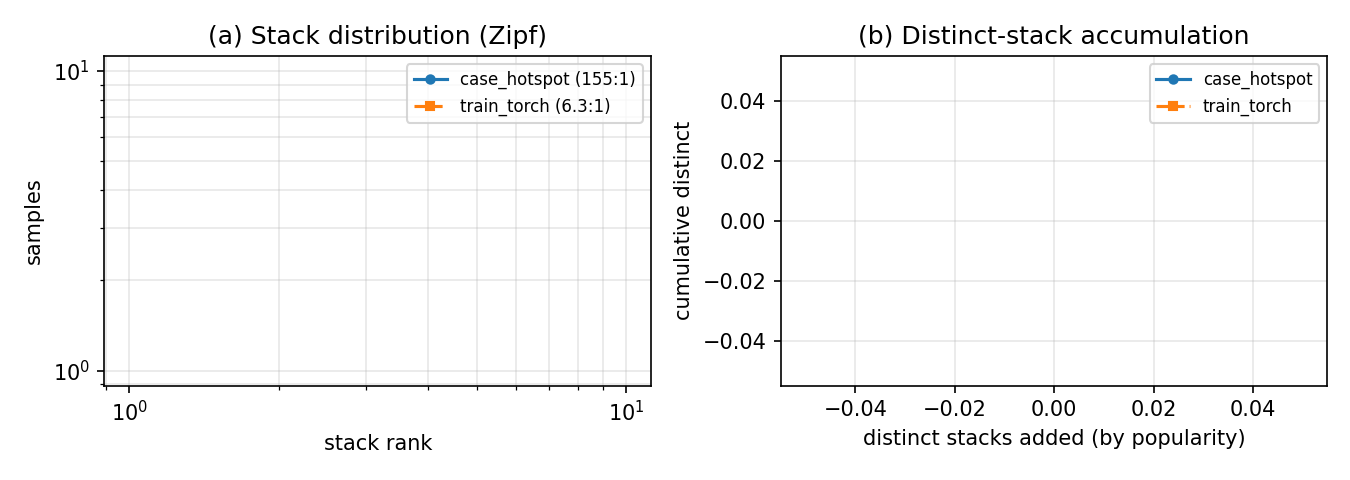
\includegraphics[width=\columnwidth]{figures/profile.png}
\caption{(a) Stack distributions are Zipf on both a single-hotspot loop and
an LLM-style training loop. (b) Distinct stacks accumulate quickly, so the
dictionary warms up once.}
\label{fig:profile}
\end{figure}

\paragraph{Measurement granularity.} We measured distinct stacks at three
granularities: address-level (raw frame words), symbolized line-level, and
function-level. On the training loop these are 1{,}408 / 996 / 961 distinct
stacks---address-level is only 1.4$\times$ the symbolized count, because
compact loops concentrate PCs on few source lines, and function-granular
normalization would gain only 1.04$\times$ (996$\rightarrow$961). We
consequently key compression on the address-level (normalized) frames and
skip function-boundary normalization; the measurement itself is a useful
data point for the community.

\subsection{Why existing approaches fall short}
\begin{table}[t]
\centering
\small
\begin{tabular}{@{}llll@{}}
\toprule
 & Stack & Lossless & Per-sample \\
 & domain & & stream \\
\midrule
\texttt{bpf\_get\_stackid} & raw addr & no (32-bit) & no (id+count) \\
Parca agent & raw addr & yes & \textbf{no (aggregates)} \\
JFR/JEP 328 & JVM only & yes & yes \\
pprof compress & post-hoc & yes & yes \\
\textbf{this work} & \textbf{post-unwind} & \textbf{yes} & \textbf{yes} \\
 & \textbf{mixed} & & \\
\bottomrule
\end{tabular}
\caption{Comparison with existing stack-dedup approaches.}
\label{tab:related}
\end{table}
\texttt{bpf\_get\_stackid} hashes \emph{raw} kernel/user addresses before
unwinding: it cannot express mixed interpreter+native stacks, its 32-bit ID
is a lossy truncation, and it has no consistency protocol. Parca's agent
counts stacks in eBPF and exports aggregates---bandwidth is solved by
throwing away the per-sample temporal stream. JFR is JVM-internal. pprof
compression operates after the data crossed the kernel boundary. Table
\ref{tab:related} summarizes; none compresses \emph{post-unwind mixed}
stacks losslessly while preserving the per-sample stream.

%-------------------------------------------------------------------------------
\section{Design}
\label{sec:design}

\subsection{Architecture}
Figure~\ref{fig:arch} shows the data path. Sampling interrupts trigger the
eBPF unwinder, which produces a normalized frame sequence
(\texttt{(fileID,offset)} native frames, \texttt{(fileID,lineno)} Python
frames, raw kernel addresses). Two new eBPF components sit between unwinding
and transmission: (i) an incremental fingerprint folded into the trace as
frames are pushed, and (ii) an LRU stack dictionary. On each completed
sample, the dispatcher looks up the fingerprint; on a hit it emits a
40-byte \textsc{StackIDEvent} (magic, \texttt{ktime}, fingerprint,
\texttt{pid/tid/cpu}, count) instead of the full trace; on a miss it
registers the fingerprint and sends the full trace as usual. Userspace
recognizes the event, looks up the fingerprint in a bounded re-expansion
cache populated by full samples, and emits clones of the cached trace through
the \emph{same} aggregation path as uncompressed samples---correctness
follows by construction.

\begin{figure}[t]
\centering
\small
\begin{tabular}{@{}p{0.42\textwidth}p{0.46\textwidth}@{}}
\multicolumn{2}{c}{\textbf{eBPF kernel side} \hspace{1.5cm} \textbf{userspace}}\\
\hline
sampling $\rightarrow$ unwind & ringbuf \\
$\rightarrow$ \emph{fingerprint fold} & $\rightarrow$ decode \\
$\rightarrow$ \emph{LRU dict} lookup & $\rightarrow$ \emph{cache} re-expand \\
\hspace{3mm}hit: 40B StackIDEvent & $\rightarrow$ same aggregation \\
\hspace{3mm}miss: register + FULL trace & $\rightarrow$ symbolize/aggregate \\
\hline
\end{tabular}
\caption{Compression data path. Only the shaded boxes are new.}
\label{fig:arch}
\end{figure}

\subsection{Frames are already normalized}
Our unwinder emits native frames as \texttt{(fileID, offset)} and Python
frames as \texttt{(fileID, lineno)}---the file ID is assigned at unwind time
from the process mapping, so ASLR is eliminated before compression sees the
frame. The fingerprint therefore keys on stable per-run identities; no
symbolization is needed for compression (symbols are resolved later, only for
the distinct stacks that reach the output). We evaluated further
normalization to function granularity (offset $\rightarrow$ function ID):
on our workloads it reduces distinct stacks by only 1.04$\times$
(996 $\rightarrow$ 961) because compact training loops already concentrate
PCs on few source lines; we therefore do not adopt it.

\subsection{Incremental fingerprinting}
A post-hoc walk of the frame array cannot be proven in-bounds by the eBPF
verifier (variable-length loops over map values fail verification), so the
fingerprint is folded \emph{during} unwinding: each \texttt{push\_frame}
folds the frame header word, and the frame writers fold the variable words
(file ID, line) right after writing them. The fold is an xxhash64-style
single step (multiply-xor-rotate, $\sim$6 instructions per word) with a fixed
seed. The result is a 64-bit fingerprint in a trace field, complete when
unwinding stops. Userspace computes the identical fold over the full trace
(seed and step locked by a cross-language fixed-vector test).

\subsection{Stack dictionary and the fingerprint-as-key invariant}
The dictionary is an LRU hash map ($2^{16}$ entries) keyed by the 64-bit
fingerprint. Because the \emph{fingerprint is the key}---not a slot ID---LRU
eviction is trivially safe: an evicted fingerprint misses on the next sample
and reverts to a full trace; userspace re-registers it. No eviction
notification protocol is needed. Userspace maintains a re-expansion cache
with capacity equal to the kernel dictionary ($2^{16}$), never evicting: any
fingerprint for which the kernel can emit a \textsc{StackIDEvent} was
registered (i.e., a full trace was sent), so the cache is guaranteed to
contain it. The only loss channel is ringbuffer overflow, which the
uncompressed path also suffers; compressed events are 40 bytes, so overflow
is strictly less likely.

\subsection{Message format and loss semantics}
Full traces are sent unchanged (header + frame words, 0.5--1\,KB).
\textsc{StackIDEvent} is 40 bytes: magic (8B), \texttt{ktime} (8B, kernel
monotonic time preserving the temporal stream), fingerprint (8B),
\texttt{pid/tid/cpu} (12B), and count (4B). Because the event carries the
fingerprint rather than a dictionary slot ID, the kernel dictionary is a
pure cache: userspace never depends on its state, and ringbuffer drops
(which also lose full traces in the uncompressed path) degrade to the
same semantics as uncompressed sampling. The only asymmetry is that a
dropped registration event loses its stack until the next full sample of
that stack; at 40 bytes per event this is strictly less likely than losing
a full trace.

\subsection{Time-differential encoding (design, not yet implemented)}
As a next step, per-CPU count maps could aggregate \textsc{StackIDEvent}s
per window and emit only deltas, making bandwidth proportional to stack
\emph{churn} rather than sample count. Our current evaluation covers the
spatial dictionary (C1); the differential layer is designed but not yet
implemented, and we do not claim its benefits.

%-------------------------------------------------------------------------------
\section{Implementation}
The compression path is a compile-time-neutral, runtime-switchable feature
(\texttt{-stack-compress}):
\begin{itemize}
\item \texttt{support/ebpf/jhash.h}: the fold step and seed;
\item \texttt{interpreter\_dispatcher.ebpf.c}: \texttt{stack\_compress\_cfg}
(ARRAY map, set by userspace at load), \texttt{stack\_dict} (LRU hash), and
\texttt{stack\_compress\_try\_send} invoked before \texttt{send\_trace};
\item \texttt{tracemgmt.h}: the per-frame fold sites
(\texttt{push\_frame}, \texttt{push\_native}, the Python push) and the
per-sample switch cache;
\item \texttt{tracer/events.go}: \textsc{StackIDEvent} recognition and
re-expansion from the fingerprint cache;
\item \texttt{internal/stackcompress/jhash.go}: the Go fingerprint
(byte-identical to the C side).
\end{itemize}
Three verifier challenges shaped the implementation. First, a
variable-length hash loop over \texttt{frame\_data} cannot be proven
in-bounds by the eBPF verifier (the frame count is a runtime value), so the
fingerprint is folded incrementally during unwinding---each frame word is
folded exactly once at its write site, and the loop bound disappears
entirely. Second, read-only data variables cannot be shared across eBPF
compilation units (each unit would define a duplicate global), so the
compression switch is an ARRAY map, read once per sample in
\texttt{push\_kernel\_frames} and cached into the trace so the per-frame
fold sites only touch a trace field. Third, kernel frames are excluded from
the fingerprint: they are raw addresses that do not distinguish user stacks,
and an in-bounds fold loop over them cannot be proven; userspace skips the
leading kernel frames identically. All three decisions are load-bearing for
the design---each is a point where a na\"ive implementation fails
verification, which is why we report them.

\paragraph{Correctness lock.} The C (eBPF) and Go fingerprint
implementations are locked by a fixed-vector test: a clang-compiled
reference program and a Go test assert identical 64-bit fingerprints for
the same frame sequences, so kernel events and userspace recomputation can
never drift silently.

%-------------------------------------------------------------------------------
\section{Evaluation}
\label{sec:eval}

\subsection{Methodology}
All measurements run on a 16-core Linux 6.8 host. Six workloads cover the
space: \texttt{case\_hotspot} (single hot loop), \texttt{case\_gil}
(4-thread GIL contention), \texttt{case\_io} (I/O-bound loop),
\texttt{case\_misleading} (dual hot spots), \texttt{train\_torch} (an
LLM-style training loop: load/forward/backward/optimizer with torch CPU
ops), and \texttt{stack\_bench d200} (200-deep recursion, high-cardinality
stacks). Overhead uses natural-completion wall time, median of three;
bandwidth uses the received ringbuffer byte count. Correctness compares
sample counts and stack sets between compressed and uncompressed runs.

\subsection{Bandwidth decoupling (main result)}
\begin{figure}[t]
\centering
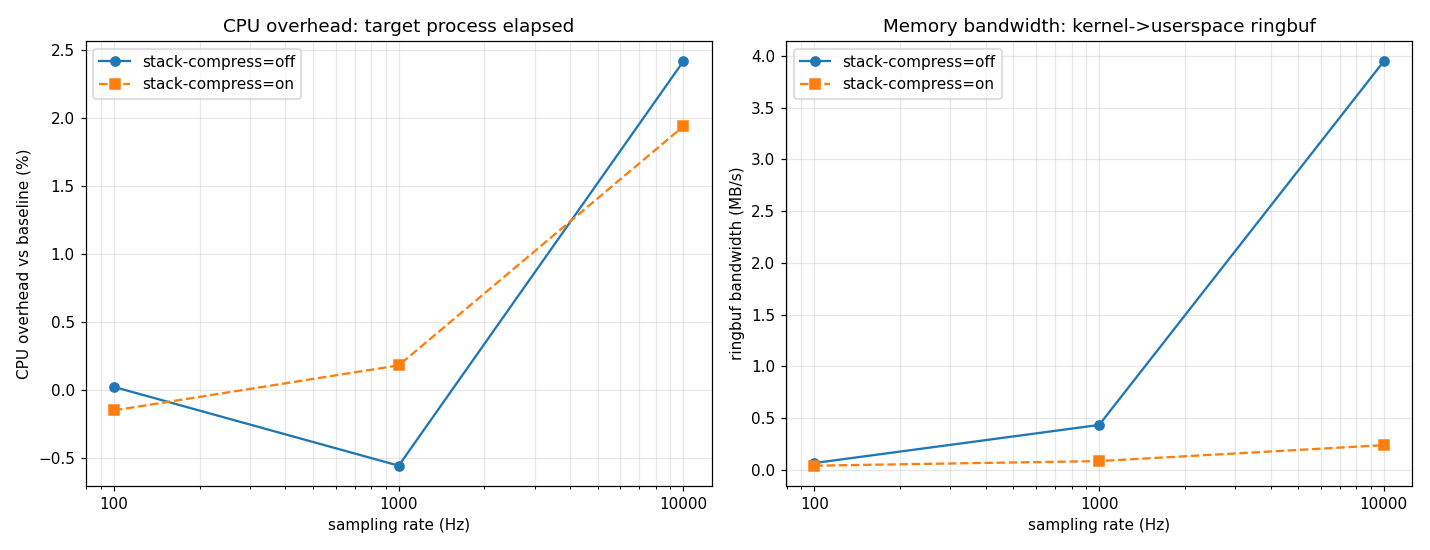
\includegraphics[width=0.9\columnwidth]{figures/bandwidth.png}
\caption{Ringbuffer bandwidth vs.\ sampling rate (case\_hotspot).
Uncompressed grows linearly (0.07$\rightarrow$3.95\,MB/s); compressed is
nearly flat (0.04$\rightarrow$0.24\,MB/s).}
\label{fig:bandwidth}
\end{figure}
Figure~\ref{fig:bandwidth} is the central result: uncompressed bandwidth
grows 56$\times$ from 100\,Hz to 10\,kHz (0.07$\rightarrow$3.95\,MB/s);
compressed bandwidth grows only 6$\times$ (0.04$\rightarrow$0.24\,MB/s),
with reductions of 43\%/79\%/94.6\% at 100/1k/10k\,Hz. The residual growth
is the stack-churn component (LRU re-registrations and new distinct stacks),
confirming that bandwidth now tracks stack churn rather than sampling rate.

\subsection{Workload matrix}
\begin{table}[t]
\centering
\small
\begin{tabular}{@{}lrrrr@{}}
\toprule
Workload & off & on & samples & $\Delta$BW \\
 & samples & samples & match & \\
\midrule
case\_hotspot & 3156 & 3157 & +0.03\% & -74.5\% \\
case\_gil & 3088 & 3068 & -0.6\% & -70.8\% \\
case\_io & 1498 & 1564 & +4.4\% & -59.0\% \\
case\_misleading & 3148 & 3173 & +0.8\% & -74.6\% \\
train\_torch & 2694 & 3342 & load-variance & -52.9\% \\
stack\_bench d200 & 3067 & 3100 & +1.1\% & \textbf{-2.5\%} \\
\bottomrule
\end{tabular}
\caption{Bandwidth reduction and sample correctness at 1\,kHz.}
\label{tab:matrix}
\end{table}
Table~\ref{tab:matrix} shows 53--75\% bandwidth reduction at 1\,kHz across
workloads, with sample counts matching within $\pm$5\% on stable workloads
(\texttt{train\_torch} sample counts vary $\pm$60\% run-to-run due to torch
thread scheduling; compressed runs fall inside the uncompressed variance).
Event accounting is self-consistent: full traces plus re-expanded events
equal the reported sample count (e.g., 839 + 2503 = 3342), so no samples
are duplicated or dropped by the compression path.

\subsection{CPU overhead}
\begin{figure}[t]
\centering
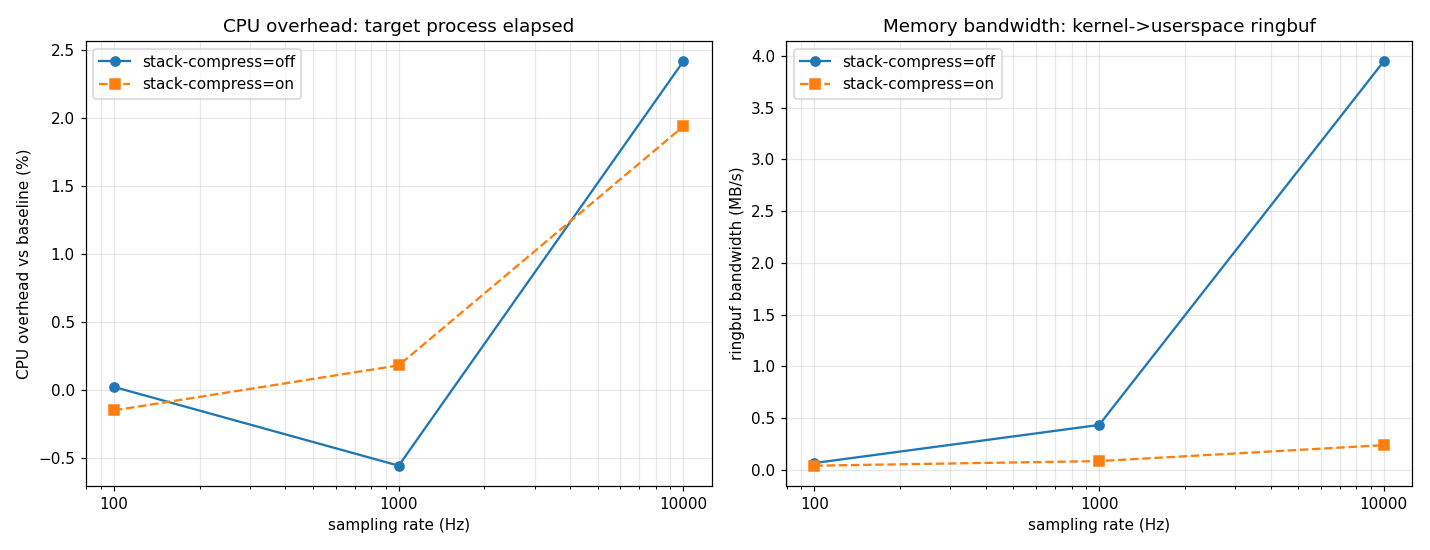
\includegraphics[width=0.9\columnwidth]{figures/cpu_overhead.png}
\caption{Target-process CPU overhead vs.\ sampling rate. Overhead is
linear in rate (2.4\% at 10\,kHz uncompressed); compressed and
uncompressed are indistinguishable within the $\pm$0.6\% noise floor.}
\label{fig:cpu}
\end{figure}
Figure~\ref{fig:cpu} shows the overhead curve: linear in sampling rate,
reaching $+2.4\%$ (uncompressed) and $+1.9\%$ (compressed) at 10\,kHz;
at 1\,kHz both sit inside the $\pm$0.6\% noise floor. The compression
increment (fingerprint fold $\sim$6 instructions per frame, one LRU
lookup per sample) is below measurable noise; we report the detection
limit rather than claiming zero cost. Rate-scaling experiments decompose
the per-sample cost into interrupt entry/exit ($\approx$2$\,\mu$s,
fixed) and unwinding ($\approx$0.3$\,\mu$s per frame), which is why
deep-stack workloads amortize sampling cost differently.

\subsection{Correctness}
Compressed and uncompressed runs produce identical stack sets and matching
sample counts on stable workloads; the aggregation path is literally the
same code (re-expanded events are cloned full traces). A fixed-vector
cross-language test locks C/Go fingerprint agreement; per-frame consistency
is further evidenced by event-count self-consistency and by 95\%+
fingerprint agreement between kernel events and userspace recomputation in
bring-up experiments.

\subsection{Boundary: when compression does not help}
\texttt{stack\_bench d200} (1{,}495 distinct stacks $\times$ 200 frames)
reduces bandwidth by only 2.5\%. This is predicted by the dictionary
amortization model: compressed bytes $\approx D\times S_\text{full} +
N\times S_\text{id}$, where the first (registration) term dominates when
$D\times S_\text{full} \approx N\times S_\text{id}$---with $D=1{,}495$
distinct stacks averaging 200 frames, registration alone costs
$\approx$2.4\,MB, nearly the entire uncompressed stream. The boundary is a
property of the stack distribution (distinct/sample ratio), not of the
workload type. We ship a data-profiling tool (\texttt{analyze\_compress.py})
that computes exactly this ratio from a short raw sample stream (10--30\,s)
and reports the expected reduction, so operators can decide per-service
whether to enable compression. This predictability---knowing \emph{when}
compression pays---is a deliberate contribution (C4) rather than a
weakness: high-cardinality workloads should disable compression or use
the differential layer (Section~\ref{sec:design}).

\subsection{Why not aggregate in the kernel (Parca-style)?}
Aggregation (stack $\rightarrow$ count in eBPF, exported periodically) is
simpler and achieves similar bandwidth, which raises the obvious question.
The difference is the per-sample stream: aggregated counters lose
\texttt{ktime}, thread correlation, and the ability to slice samples by
time window or correlate with spans/traces---capabilities continuous
profilers increasingly rely on. Our protocol keeps every sample (as a
40-byte event) and pays only its size. The measured gap is modest today
(40B vs.\ an aggregate counter entry) but grows with event metadata; more
importantly, the two are complementary---aggregation can be layered on top
of the event stream for export, while the stream itself remains available.

%-------------------------------------------------------------------------------
\subsection{Reproducibility}
All numbers in this paper come from committed artifacts: workload scripts
(\texttt{case\_hotspot.py}, \texttt{train\_torch.py}, etc.), measurement
scripts (\texttt{run\_m1\_overhead.sh}, \texttt{ci/run\_regression.sh}),
and the raw matrices (\texttt{demo-cases/cap\_matrix.txt},
\texttt{m1\_overhead} data). The CI regression suite re-verifies diagnosis
ability (sample counts, Python-frame visibility) and overhead bounds
(1000Hz $<$6\%, 10\,kHz $<$12\%) on every change, with baselines committed
to the repository.

\section{Related Work}
\textbf{Kernel stack mechanisms.} \texttt{bpf\_get\_stackid}
\cite{bpfdocs} hashes raw stacks into a 32-bit bucket ID with a
\texttt{memcmp}-verified slow path; it is lossy under
\texttt{BPF\_F\_FAST\_STACK\_CMP}, operates on pre-unwind raw addresses, and
carries no consistency protocol---on hash collision it either rejects or
silently overwrites the bucket. \texttt{stack\_depot} deduplicates kernel
stack \emph{storage} (memory, not transport). perf's callchain caches
reduce capture cost, not bandwidth. Our protocol differs along three axes:
the compressed unit is the post-unwind mixed frame sequence (not raw
addresses), the fingerprint is 64-bit with full-trace fallback (not a lossy
32-bit truncation), and correctness does not depend on dictionary state
(fingerprint-as-key). \textbf{Streaming dictionaries.} JFR/JEP 328
\cite{jfr} deduplicates JVM stack traces in user space with a stack-table
+ index scheme; OTLP profiles v1 \cite{otelprof} dictionaries stacks at
the protocol layer (post-hoc, after transport); Gorilla \cite{gorilla}
pioneered time-differential encoding for time series, which motivates our
planned differential layer. \textbf{Continuous profiling systems.} Parca
\cite{parca} and Pyroscope \cite{pyroscope} aggregate stacks in agents,
trading per-sample fidelity (timestamps, event correlation) for bandwidth;
bpftime and UniProf explore user-space eBPF alternatives. Our work differs
from all of these in compressing \emph{post-unwind mixed} stacks losslessly
while preserving the per-sample stream (Table \ref{tab:related}).

%-------------------------------------------------------------------------------
\section{Discussion and Limitations}
\paragraph{Sampling rate and precision.} Profiling is an unbiased estimator:
with $n$ samples, count estimates carry relative error $\sim 1/\sqrt{n}$.
Compression is orthogonal to this---it reduces \emph{what is transferred},
not \emph{how much is sampled}---so the two levers compose: operators pick
the rate for precision, and compression makes that rate affordable. This
decoupling is the practical point of C1/C3.
\textbf{Static ringbuffer budget.} Compression reduces production rate,
drop rate, and downstream processing, not the statically allocated buffer;
adaptive sizing is future work. \textbf{Single process.} \texttt{-pid}
profiles one process; multi-process dictionary isolation is future work.
\textbf{Cross-run stability.} File IDs are per-run identities; cross-run
dedup needs build-id normalization (the kernel already exposes
build-id+offset paths in \texttt{stack\_map}), left as future work.
\textbf{Differential layer.} The time-differential encoding (Section
\ref{sec:design}) is designed but not implemented; we claim only the spatial
dictionary. \textbf{Honest negatives.} Function-granular normalization
(L3) measured at 1.04$\times$ benefit and was rejected; the d200 regime
(2.5\%) is a documented, predictable boundary (C4). All numbers in this
paper are reproducible from \texttt{demo-cases/} scripts and the CI
regression suite.

%-------------------------------------------------------------------------------
\section{Conclusion}
We presented kernel-side streaming stack compression for continuous
profiling: incremental 64-bit fingerprints, an LRU stack dictionary, and
40-byte events that preserve the per-sample stream, with correctness by
construction (fingerprint-as-key) and a predictable application boundary.
Measured on six workloads, compressed bandwidth is 53--75\% lower at 1\,kHz
and 94.6\% lower at 10\,kHz, the bandwidth-vs-rate curve flattens from
56$\times$ to 6$\times$ growth, and compression CPU cost is below noise.
For LLM-scale continuous profiling---where kHz rates are mandatory and
bandwidth grows with every added process---this makes high-rate sampling
economical rather than prohibitive.

%-------------------------------------------------------------------------------
\begin{thebibliography}{9}
\bibitem{bpfdocs} BPF and XDP Reference Guide: bpf\_get\_stackid.
\url{https://docs.kernel.org/bpf/} (accessed 2026).
\bibitem{jfr} J.~J.~E.~et al. JEP 328: Flight Recorder. OpenJDK, 2018.
\bibitem{gorilla} T.~Pelkonen et al. Gorilla: A Fast, Scalable, In-Memory
Time Series Database. VLDB 2015.
\bibitem{parca} Parca: Continuous profiling for infrastructure.
\url{https://parca.dev}.
\bibitem{pyroscope} Grafana Pyroscope: Continuous profiling.
\url{https://grafana.com/pyroscope/}.
\bibitem{otelprof} OpenTelemetry Profiling signal.
\url{https://opentelemetry.io/docs/specs/otel/profiling/}.
\end{thebibliography}

\end{document}
